\setchapterpreamble[u]{\margintoc}
\chapter{Machine Learning \& Computer Vision}
\labch{MLandCV}
In this chapter the theoretical backgrounds and motivation of neural networks ought to be explored.

First, a physical/biological motivation will set the foundation for the theoretical background accompanied by a more mathematical motivation later on.
Thereafter, more advanced lines of thought will be introduced that finally lead to convolutional neural networks as the current driving force in computer vision.

\section[Artificial NNs]{Artificial Neural Networks}

\subsection[Inspiration]{Neurobiological Inspiration}

Many human achievements have at least been partially inspired by studying nature.
A very popular example is that of airplanes and birds.
By studying how birds can fly, people found out that the shape of their wings is essential.
Inventors and engineers have taken this as inspiration and slowly but steadily came up with planes and the like.
However, planes are not birds, as they are not flapping their wings (yet?), but in combination with other inventions like jet engines, the obtain the same (or better) capability of flying like birds.

Similarly, the brain features a lot of insights, how intelligence or something that seems like it can be modeled.
In the same way, that humans studied birds to understand flying, researchers are now studying the brain to create better artificial intelligence.

In the earliest stages of this research, they would try to imitate the brain, as people have tried imitating birds at first; and they failed similarly.
\begin{figure}
    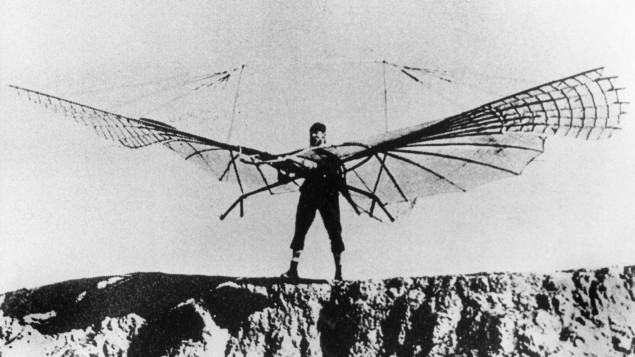
\includegraphics{otto_lilienthal}
    \caption[]{Otto Lilienthal with his flying apparatus. One example of how people failed in trying to imitate nature too closely. \url{https://www.deutschlandfunkkultur.de/geschichte-der-fliegerei-wie-der-mensch-die-voegel.976.de.html?dram:article_id=308043}}
    \labfig{lilienthal}
\end{figure}
\marginnote{There is current research on replicating the brains structure to the neuron level on hardware with more success \cite{brainscales}.}

Warren McCulloch and Walter Pitts proposed one of the earliest models of an artificial neuron.
They aimed at simplifying models of a biological neuron at the time.
\marginnote{Notably McCulloch and Pitts (1943) even preceded Hodkins and Huxley's (1952) Nobel price winning description of a neuron.}

\subsubsection{Biological Neuron}
For this reason, the functioning of a neuron shall be described shortly.

Human cells that make up the brain are called \textbf{neurons}.
They connected through dendrites, synapses, and axons.
These connections allow neurons to exchange signals with other neurons.

A neuron receives signals through its dendrites, which all lead to the cell body (soma).
The cell body accumulates these signals.
If the summed value of the signals' potentials reaches a certain threshold, an action potential (spike) is generated.
The spike then travels as a signal along the axon and its branches towards other neurons.
Axons end in synapses that connect to other neurons' dendrites.
Synaptic transmissions are usually mediated by chemicals and not by electrical signals.
The chemical nature of the synapse allows it to forward either an excitatory or an inhibitory signal.
Excitatory signals will bring the cell potential closer to the threshold, while inhibitory do the opposite \cite[p.~42]{coloratlas}.
\marginnote{Cell potentials are decreases by excitatory signals, as the action threshold sits below the resting potential.}

What makes the brain so powerful, though, is not the neuron itself with its arguably simple structure but the vast network of billions of these neurons.
Each neuron is connected to thousands of other neurons with which it communicates.
How a signal is transported between neurons depends on the interplay of synaptic weights, neural connections, and the threshold of each neuron.

\subsubsection{Artificial Neuron}
McCulloch and Pitts saw that powerful things could be achieved when connecting lots and lots of simple structures.
Thus, they proposed an even simpler model of a neuron: \\
They restricted their neuron to a binary state (on or off).
Each neuron gathers signals from other neurons, which are either positive or negative.
A neuron only becomes active if the number of incoming positive signals minus the number of negative signals exceeds the neuron's threshold.
\todo{add equation with activation function, when neuron fires}
McCulloch and Pitts then also changed the highly parallel and complex nature of biological neural networks to a single layer feed-forward network architecture.

In a feed-forward network, neurons are grouped into layers and operate in parallel within a layer.
They do not interact within a layer.
Each neuron in a layer is fed the same input signal (often described as an input layer).
The neuron's state is then computed according to an equation such as \refeq{mcculloch}.
The activation value of each neuron then defines an output.

As this model deviates from nature quite a bit, these structures a better referred to as \textbf{units} instead of neurons.

In a single layer architecture, a layer often consists of a single unit (see \reffig{ff_arch}.
Basically, input signals come from one side, and output signals go out the other side, which can be expressed in a simple equation like \refeq{mcculloch}.
This is not only done for practical reasons but also inspired by the observation of layered neuron structures in the brain.

The McCulloch-Pitts model is capable of emulating simple logical relations (\lstinline|AND|, \lstinline|OR|, \lstinline|NOT|) but nor \lstinline|XOR| which will be explained later.

\subsubsection{Perceptron}
This McCulloch's and Pitts' is very much simplified yet comes with some weaknesses.
Thus, the \textbf{perceptron} has been introduced by Frank Rosenblatt in 1957.
Instead of having a binary unit, he came up with a linear threshold unit (LTU).
The LTU allows for numeric instead of binary signals, which can be weighted with independent factors.
Also, a unit's threshold/bias is parameterized as another weight with a constant input using the 'bias trick'.
The resulting equation for each LTU then reads:
\todo{equation for LTU with bias trick}
Equation \refeq{LTU} can then be formulated in a vectorized form such that:
\todo{vectorized LTU}

In this form, the calculations for each unit become mathematically and computationally relatively easy.
Each layer can be expressed as a vector of activations $\vec{x}$.
Multiplying this vector with the weight matrix $\mat{W}$ and applying the element-wise activation function returns the activations for the subsequent layer.\\
\marginnote{The word perceptron describes the whole function $f$ in equation \refeq{perceptron} which can consist of many LTUs}
%simplified computational model of how biological neurons might work together
This capable yet straightforward description of a unit built the base for the first surge of interest in neural networks (connectionism).

\subsubsection{Mathematical Interpretation}
The simplistic mathematical formulation of the perceptron suggests that there might be a mathematical meaning besides the biological analogy.
Indeed, the perceptron is equal to the definition of a \textbf{binary linear classifier}.

A binary linear classifier categorizes inputs into two classes, hence binary.
It does so by drawing a virtual hyperplane in input space and predicts the class for each input.
The decision depends on whether a point lies above or below this hyperplane.
\begin{marginfigure}
    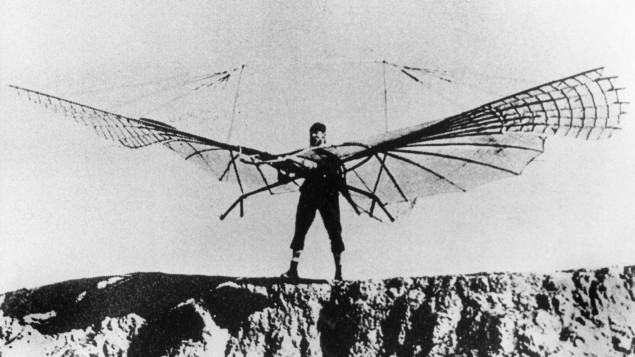
\includegraphics{otto_lilienthal}
    \caption[]{As a simple example, this binary classifier has data on how often the words 'weight loss' and 'invest' appear in an email.
Any time these two words appear too often, the data point is above the decision boundary. An email is then classified as 'spam'}
    \labfig{linear_class}
\end{marginfigure}
As the hyperplane (or decision boundary) is quantified by a linear function, the classifier is described as linear.

A classic problem would be classifying email as spam.
Given two data inputs (\ie frequency of the words 'weight loss' and 'invest'), the classifier has to make a decision.
For this reason, the binary classifier defines a \textbf{decision boundary}.
Any data point that lies above this decision boundary is classified as 'spam', any point beneath is classified as 'not spam'
Since regular emails rarely use the two words, they do not classify as spam.\\
Other people \ie nutritionists, on the other hand, will have the word weight loss come up more frequently.
This means the decision boundary must differ for different users and their mail.

To compute where a point lies relative to the decision boundary, a data point's value along each axis $x_1, x_2$ is weighted individually $w_1, w_2$, and summed with a bias $b$.
The result is checked whether it is above or below a threshold $t$.
\begin{align}
    z = w_1 x_1 + w_2 x_2 + b
\end{align}
With the classification 'spam' if $z > r$ and 'not-spam' $z \leq r$ (\textit{in dubio pro reo}).
Equally $z - r > 0$ holds for spam as well such that the threshold can be brought into the equation and $z$ is checked against $0$.
$r$ can then be absorbed into the bias.
\begin{align}
    \rightarrow z = w_1 x_1 + \hdots + w_D x_D + b - r = w_1 x_1 + \hdots + w_D x_D + b'
\end{align}

For arbitrary dimensions $D$ this becomes
\begin{align}
    z = w_1 x_1 + \hdots + w_D x_D + b
\end{align}
 where $\vec{x}$ and $\vec{w}$ can be defined by vectors
\begin{align}
    z = w_1 x_1 + \hdots + w_D x_D + b = \vec{w}^T \vec{x} + b
\end{align}
The decision boundary can be easily derived from this, since $\vec{w}$ is the orthogonal vector to the hyperplane and $\frac{b}/\norm{\vec{w}}$ is the displacement of the plane along $\vec{w}$.

For a simpler notation, one can define an additional 'virtual' input which has a constant value of $1$ as $x_0$, the bias $b$ can then be elegantly included into $\vec{w}$ (same 'bias trick' as before)
\begin{align}
    z = w_0 b + \vec{w}^T \vec{x} = w_0 b + w_1 x_1 + \hdots + w_D x_D = \vec{\hat{w}}^T \vec{x}
\end{align}
with $x_0 = 1$ and $w_0 = b$.
The output $z$ can also be seen as a function of $x$.
Then, $w$ can describe any function linear in $f$.
%\todo{explain ability to imitate any linear function.}

This description also holds for perceptrons with more than one unit.
In that case, the input vector $\vec{x}$ and the weights $\vec{w}$ become matrices with multiple column vectors.
\begin{align}
    \vec{x} \rightarrow (\vec{x}_1, \vec{x}_2, ...) = \mat{X}
    \vec{w} \rightarrow (\vec{w}_1, \vec{w}_2, ...) = \mat{W}
    \rightarrow \vec{z} = \mat{\hat{W}}^T \vec{X}
\end{align}


\subsubsection{Loss Function}
With a mathematical definition at hand, the next step is to quantify the output.
In order to train a classifier, an objective has to be formulated through a \textbf{loss function}.
Usually, there is already a data set for the network to train on.\\
In the given example this would be mails which were read beforehand and then declared either 'spam' $\tilde{y}_i = 1$ or 'not-spam' $\tilde{y}_i = -1$
$\tilde{y}_i$ is called the \textbf{label} for a sample $x_i$ with index $i$.

With the binary linear classifier, the decision boundary has been introduced (check $z_i > 0$) to predict a label for any given sample.
This is sufficient to predict a class, but much information is lost this way.
For training and evaluation, the information available in $z$ should be used.\\
\eg, a large $z_i$ implies that the data point $x_i$ sits far from the decision boundary.
Thus, the classifier is very sure of this classification.
For $z_i \approx 0$, the classifier is not that sure, and for $z_i = 0$ the classifier is indecisive.
Ultimately, $z_i$ can be seen as a score that is calculated for each data input.

The question then becomes how to quantify how well the classifier performs on given data.
Hence, a loss function is defined, which measures the classifier's performance on the data.
A popular choice is \textbf{least squares}, where the score's distance to the label is measured.
\begin{align}
    \L_{\text{LS}} = \sum_i (y_i - z_i)^2
\end{align}
The value of the loss function becomes minimal for $y_i = z_i, i = 1,...,N$.
Yet, this score function is especially susceptible to outliers which will cause the decision plane to skew towards outliers with $z_i > 1$ or $z_i < -1$

For this reason \textbf{support vector machines (SVM)} employ a \textbf{maximum margin} classifier.\\
A maximum margin classifier seeks to find a decision boundary which is as far from the closest representatives of each class as possible (see \reffig{SVM}).
The maximum margin is defined as
\begin{align}
    \text{margin} = d_+ + d_-
\end{align}
with $d_+$ the distance to the nearest training sample with class $+1$ and $d_1$ to closest training sample with class $-1$.
Noticeably, this requires the data to be linearly separable, which means that a hyperplane must exist that perfectly separates the data according to its class.
The margin becomes ideal for $d_+ = d_-$.
Since $w$ is orthogonal to the hyperplane, $\vec{w}$ can always be rescaled such that 
\begin{align}
    d_+ = d_- = \frac{1}{\norm{\vec{w}}}
\end{align}

Additionally, $\vec{w}$ can be chosen such that $z = \vec{w}_i^T \vec{x}_i + b_i \geq +1$ for $\tilde{y}_i = +1$ and vice versa for $\tilde{y}_i = -1$.
Thus,
\begin{align}
    \tilde{y}_i z_i \geq 1
\end{align}
will hold, for all inputs $x_i$ with equality for points on the margin, as there is always at least one point of each class on the margin.

Thus,
\begin{align}
    d_- = d_+ = \frac{1}{\norm{\vec{w}}}
\end{align}
and the margin
\begin{align}
    d_- + d_+ = \frac{2}{\norm{\vec{w}}}
    \labeq{maxmargin}
\end{align}
is maximized when $\norm{\vec{w}}$ is minimized.

Subsequently, the classification can be expressed as a relatively simple optimization problem.
\begin{align}
    \argmin_{w, b} \frac{1}{2} \norm{\vec{w}}^2
\end{align}
under the constraints
\begin{align}
    \tilde{y}_i z_i = \tilde{y}_i (\vec{w}_i^T \vec{x} + b) \geq 1 \forall i
    \labeq{constraint}
\end{align}
How to solve this optimization problem shall be explained in \refssec{svmopt}.

\subsection{Regularization}
Regularizations, combined with loss functions, penalize possible solutions deemed wrong for any particular reason.
A very common regularization is L2 regularization on the weights.
It is expected that networks with very large weights generalize poorly.
Hence, all weights are summed up and multiplied with a regularization constant $\lambda$ \cite{grosse}.
\begin{align}
	\mathcal{R} = \frac{\lambda}{2} \sum_{i = 1}^D w_i^2
\end{align}

\section[Fully Connected NNs]{Fully Connected Neural Networks}
\subsection{Multi-Layer Perceptron}
With the perceptron, which is capable of classification any linear separable data, at hand, the question becomes: What are the limitations to this?
Minsky and Pappert found the limitations in 1969 with their book 'Perceptrons'.
They oulined the limitations of perceptrons with the \lstinline|XOR| problem \cite{perceptron}.
The problem becomes obvious when looking at the \lstinline|XOR| problem in a 2D plane (see \reffig{XOR})
\begin{marginfigure}
    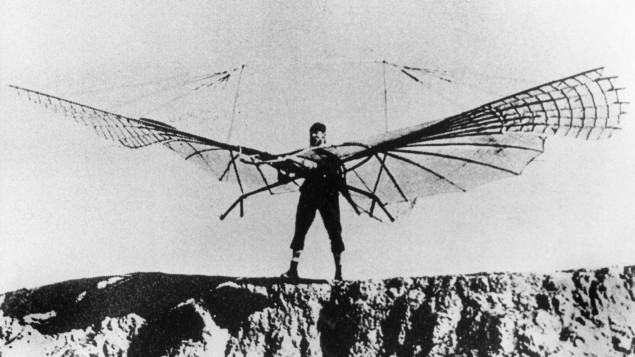
\includegraphics{otto_lilienthal}
    \caption[]{\lstinline|OR| and \lstinline|XOR| operations visualized. The \lstinline|XOR| problem cannot be solved by drawing a single line.}
    \labfig{XOR}
\end{marginfigure}

As it has been explained in the previous section, the perceptron is equal to a binary linear classifier.
As such, the perceptron can only classify linear separable data perfectly.
Since the \lstinline|XOR| problem can obviously not be solved with a straight line separating the two classes, the perceptron is also not able to compute such an operation. 

This realization led to the first decline in interest in artificial neural networks.

Since then, there have been ways of solving this problem for SVMs by projecting the data into a higher dimensional space with various kernel functions \cite{ommer}.
Another approach keeps the logic but goes from the shallow network approach to a deep neural network (DNN).
\textbf{Deep Neural Networks (DNN)} are ANNs which consist of more than one hidden layer.
A single perceptron may not be capable of computing \lstinline|XOR| but it is capable of calculating \lstinline|AND|, \lstinline|OR| and their negated forms.
By using one perceptron with two units to compute \lstinline|AND| and \lstinline|OR|, a second layer perceptron can in fact compute \lstinline|XOR|
\begin{align}
    XOR(x, y) = AND(OR(x, y), NOT(AND(x, y)))
\end{align}

Thus, DNNs solve the \lstinline|XOR| problem.

\marginnote{The ability to stack \textit{and train} multiple layers in ANNs stems from the discovery of backpropagation which shall be explained in \refssec{backprop}.}

Perceptrons, until then, could approximate only linear functions.
Multiple layers of perceptrons now promise to approximate any higher degree function just as well.
Thus, \textbf{Multi-Layer Perceptrons (MLP)} sparked new interest in the field of artificial neural networks.

This interest also originated in the similarly layered structure that has been found in the brain.
\begin{marginfigure}
    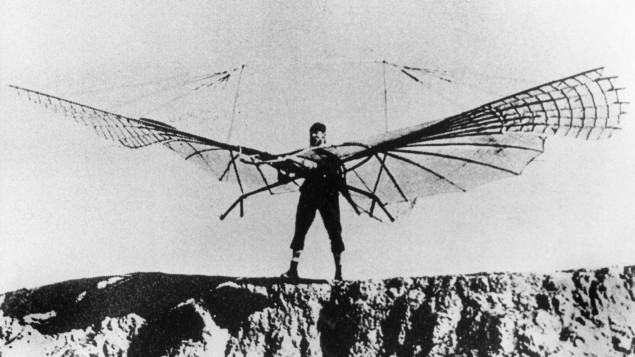
\includegraphics{otto_lilienthal}
    \caption[]{The brains structure under a microscope}
    \labfig{brain}
\end{marginfigure}
\begin{marginfigure}
    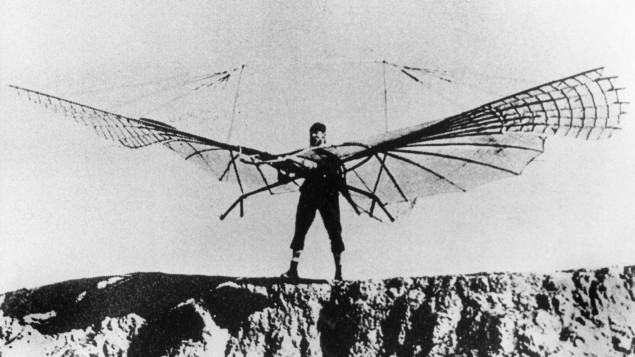
\includegraphics{otto_lilienthal}
    \caption[]{Layers of an MLP}
    \labfig{MLP}
\end{marginfigure}
Ultimately, MLPs really start to show the connected structure in a network that is typically expected.

MLPs are also called \textbf{fully connected networks} since each unit is connected to all unit in the previous layers as well as all units in the next layer.

%\marginnote{This new connectedness opens a realm to a whole field of studies on graphs, networks and network motifs \cite{network_motifs}.}

%histrocal rollercoaster of interest (AI winter) ?
%limited capabilities of the perceptron for XOR problem
%use either higher dimensional input -> kernel trick or stack many perceptrons
%any 2 layer MLP can approximate any continuous function (or somethign like that)
%simialrity to network motifs, make a large network of many identical pieces
%similar to how the brain works as well.

\subsubsection{Activation Functions}
%linear algebra shows that any linear function can approximated by just two perceptron layers for a linear activation function -> more layers do not make sense.
These newfound capabilities for MLPs are not only restricted to binary operations but will translate into continuous space.
In this case the hidden-layer perceptrons get stripped of their activation function.
The activation function of a perceptron has been used, up until now, to make a class prediction $y_i$ from a score $z_i$, which is also called pre-activation~\cite[p.~6]{GrosseNotes}.

Replacing the step function with a linear activation function (\ie identity function), each hidden-layer's perceptron would initially seem to increase the capabilities of the MLP.
Unfortunately, this is not the case as any subsequent perceptrons with linear activations can be reduced to a single preceptron.
\begin{align}
    \vec{z}_2 = \mat{W}^T_2 \vec{z}_1(\vec{x}) = \mat{W}^T_2 \mat{W}^T_1 \vec{x} = \mat{W}' \vec{x}
    \labeq{LAF}
\end{align}

Consequently, the step-function that was used in the \lstinline|XOR| problem played an important role.
The reason for this is the non-linear nature of the step-function in contrast to any linear activation function.
It can easily be shown that \refeq{LAF} does not hold if a non-linear activation function is used.

Thus, the question becomes which other activation functions there are that go beyond binary classification.
An early popular choice was sigmoid functions (logistic function or $\tanh$).
Especially the logistic function is popular due to its similarity to the step-function amongst other things.
\begin{align}
    \sigma(z) = \frac{1}{1 + e^{-z}}
\end{align}
\begin{marginfigure}
    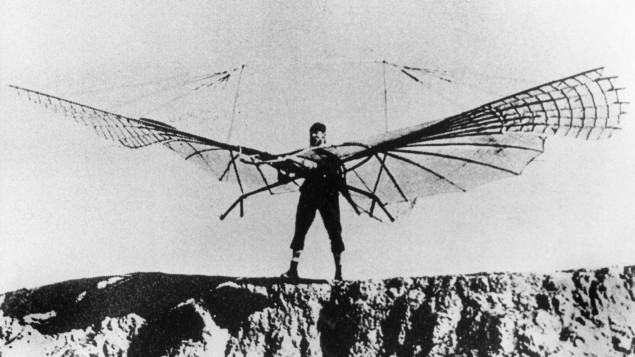
\includegraphics{otto_lilienthal}
    \caption[]{A sigmoid function. It saturates to $1$ for very large inputs and $0$ for very small inputs, similar to the step function.}
    \labfig{sigmoid}
\end{marginfigure}

Another popular choice are rectified linear units (ReLU) which are identical to a linear activation for $z > 0$ but mimic the step function for $z < 0$.
Basically, a ReLU suppresses the signal of a perceptron until it reaches the threshold of $0$ and then forwards the signal unaltered.

Another activation function 'leaky ReLU' attenuates the signal below the threshold with a factor $\alpha$ instead of fully suppressing it.
\begin{marginfigure}
    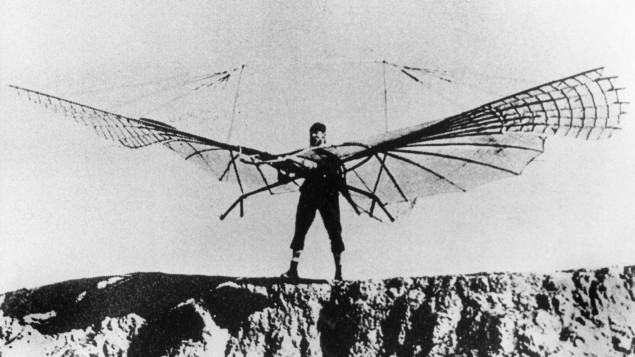
\includegraphics{otto_lilienthal}
    \caption[]{ReLu activation function}
    \labfig{relu}
\end{marginfigure}
\begin{marginfigure}
    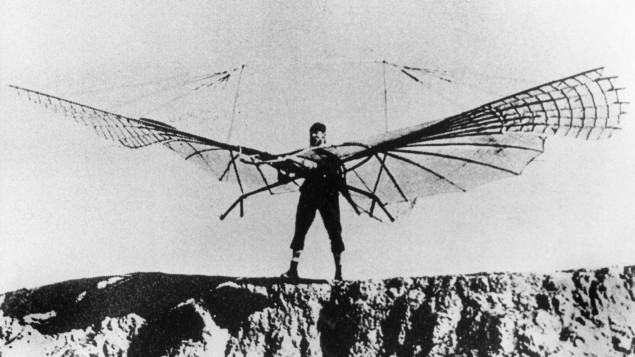
\includegraphics{otto_lilienthal}
    \caption[]{leaky ReLu activation function with $\alpha = 0.2$}
    \labfig{lrelu}
\end{marginfigure}

\section[Convolutional NNs]{Convolutional Neural Networks}
With fully connected networks at hand, it seems as if any complex function could be solved by just stacking enough hidden layers.\\
While this seems compelling at first, the issue of the computational burden arises very quickly.
Especially for broad layers with many units the number of connections and weights becomes problematic.
For two exemplary layers with $1,000$ units each, there would be $1,000,000$ connections as well as $1,000$ biases.
This causes two kinds of problems.
\begin{enumerate}
    \item Each connection represents a multiplication and summation to the activation value with an associated computational cost.
    \item All connections have separate weights which must be trained, which requires a vast number of training data.
\end{enumerate}

Another problem is invariance for spatially or temporally distributed data.
If a pixel is to be shifted by a single pixel, or an audio track delayed by a second, the content does not change, and as such the result should not either.
An FCN would likely over-fit the data and be susceptible to such variations.

Computer vision as a field is particularly affected by this issue.
Since the input are often images with upwards of $64 \times 64 = 4096$ pixels.
Hence, a different solution is needed.

\subsection{Convolutions}
A solution to the previously stated problem are convolutional layers.

A \textbf{convolution} is a mathematical operation which produces for any given point of a function $f$ the weighted average of its surroundings.
The way the surroundings are weighted is through a kernel function $g$.
This principle can be translated into image space where a filter $g$ is applied to each pixel and its surroundings.\\
\marginnote{A convolution is commutative $f * g = g * f$, associative $f * (g * h) = (f * g) * h$ and distributive $f * (g + h) = f * g + f* h$.} 
Specifically, many filters of size $k \times k$ are put on top of the image similar to tiles on a roof.
Tiles may overlap but are evenly spaced over the area they cover.
The spacing between the centers of each tile is called a stride $s$ and will be assumed the same along each dimension.
The return value of each filter then defines a new grid of values much like the original input.
Typically, the output of such a convolution is smaller than the input, since the outermost filter must still fit fully into the image.
Yet, it is possible to avoid this problem by padding an image with values such that the output has the same size.

These filters may seem very simple but they are able to capture very interesting properties in an image and transform them as well.
\begin{marginfigure}
    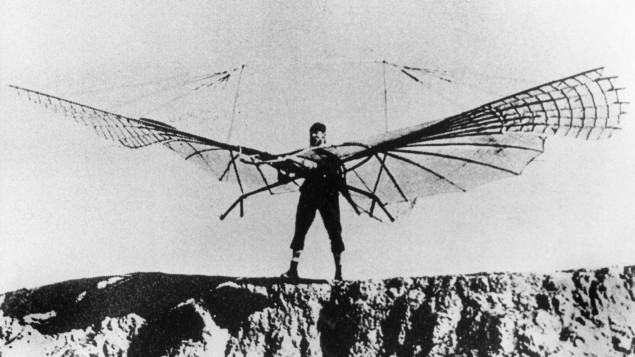
\includegraphics{otto_lilienthal}
    \caption[]{A convolution in 1D space}
    \labfig{conv}
\end{marginfigure}
The easiest example would be a 3x3 filter which blurs the image it is applied to.
The filter given in \reffig{conv_blur} results in such blurring since the signal of the pixel at the center is dominant but mixed with the signal of its surrounding pixels.
\begin{marginfigure}
    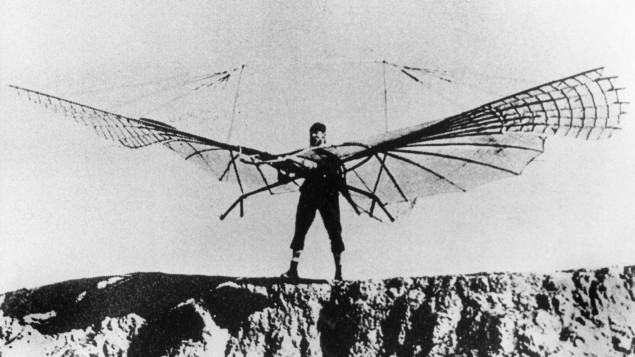
\includegraphics{otto_lilienthal}
    \caption[]{3x3 filter for blurring.}
    \labfig{conv_blur}
\end{marginfigure}

Another filter like \reffig{conv_sharp} will sharpen edges in an image since the signal of the surrounding pixels is subtracted from at the center pixel signal. 
\begin{marginfigure}
    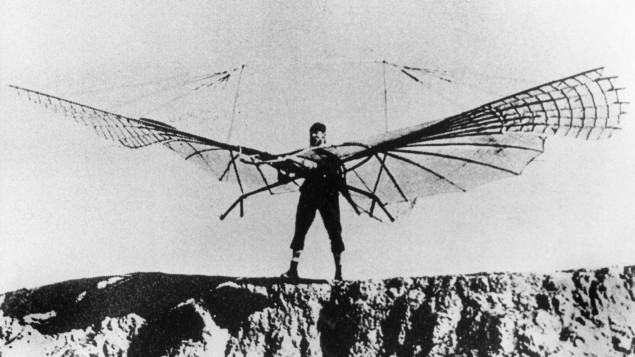
\includegraphics{otto_lilienthal}
    \caption[]{3x3 filter for sharpening edges.}
    \labfig{conv_sharp}
\end{marginfigure}

One can easily imagine that these kernels can also perform blurring only along one axis or sharpening gradients in one direction.
As many such filters are imaginable, there are often many filters applied per layer called filter-banks.
The output of each filter then defines an input channel for the next layer much like the three color channels in an image.
With many channels convolutions can become even more complex as each filter takes all previous channels as input and combines them into a new channel.\\
Interestingly, the weights of each kernel may not be hand-crafted but can be learned similar to fully connected layers.

As convolutions qualify as linear functions, there exists an equal fully connected layer to each convolutional layer.
The weights of such an FC layer would be sparse, though, which means there are many values equal to zero.
This property makes it clear that convolutions are more efficient than fully connected layers by imposing some simple restrictions.

Similar behavior also occurs when comparing convolutional layers with different kernel sizes.
By using a larger kernel, the 'field of view' (the area that each pixel in the result layer 'sees') increases as well.
At the same time, a larger kernel increases the number of parameters significantly.
\marginnote{A convolutional kernel with the size of the input would be equivalent to a fully connected layer.}
The same field of view can also be obtained, though, when using two convolutions in series.\\
\eg two layers with kernel size $3 \times 3$ have the same field of view like a single layer with kernel size $5 \times 5$ but fewer weights.

\subsection{Pooling}
A sub-type of convolutional layers are pooling layers.
Pooling layers have the purpose of downsampling an image or layer to a lower resolution.
Basically, downsampling can already be achieved by choosing a convolutional layer with stride $s > 1$.
Another way is to downsample an image without any learnable weights is by using one of two specific hand-crafted kernels.

The first option is average-pooling.
By taking the mean of four neighboring pixels (each weight is $\frac{1}{4}$) with a stride of $s = 2$ in each channel, the input is scaled down by a factor of $2$ along each axis.
Figuratively, four pixels will be combined into a single pixel by taking their mean.

On the other hand, max-pooling does not take the average but only takes the maximum value of the four inputs.
The result will then propagate only the most dominant signals.

Either way, pooling will result in loss of information but is often necessary to reduce the computational load.
Especially when the number of channels increases for deeper layers, it is preferable to reduce memory usage and computational load along with the spatial size.

Typical CNN architectures will often stack several convolutional layers then apply a single pooling layer.
Then another stack of convolutional layers is applied.
This way, the input's spatial size is gradually reduced, while the number of channels is increased at the same time.

\section{Recurrent Neural Networks}
imprtant to generate sequences
more efficient than just predicting everything at once
speech is good example: first word matters for the next few words, but the first word a few senteces ago is mostly irrelevant
\subsection{Long-term Short Memory}
LSTM is a substructure
expalin and show iamge


\section{Types of Learning}
types of training are not clearly separated, there is weakly supervised training and the like
more or less categorizes networks by their setups a.k.a. how they learn.
most application fall in this category
straight forward
classify this, generate this

\subsection{Supervised Learning}
GIve a predefined problem and tell the network which metric to look for and how to solve the problem

\subsection{Reinforcemnt Learning}
No loss directly but a score is given to evaluate performance
loss would be differentiable
e.g. game: loss cannot be calcualted but a score can be given at the and or in between
Reinforcement learning is employed when there is a lack of gradients at some point in the pipeline.
A very well known example are AIs which play computer games.
The interaction with a game happens through a predefined interface which is usually not differentiable.
This has two main reasons:
\begin{enumerate}
    \item Humans or algorithms do not need a differentiable interface with a computer game.
    \item It is very hard to think of a way to make an action like moving a figure in chess differentiable.
\end{enumerate}

Yet, AIs like Google Alpha Go are based on neural networks.
Reinforcement learning allows for this as is introduces learning techniques that formulate ...

\subsection{Unsupervised Learning}
Just give a bunch of data and see whether it can be ordered or represented in an efficient way
Usually there is still an intention but its not that narrow

